\documentclass[UTF8]{csoarticle}


\newtheorem{theorem}{定理}
\newtheorem{lemma}{引理}
\renewcommand{\proofname}{证明}
% 如果为英文文章,可以使用下面的定义(去除行首的注释符号%)代替上述中文定义
% \newtheorem{theorem}{Theorem}
% \newtheorem{lemma}{Lemma}

\begin{document}

%----------------------------------------------------------
% 1. 文章标头信息
%----------------------------------------------------------

\titleCHN{文章的中文标题}
\titleENG{Title of article}
\authorCHN{张三丰\affil{1},李四\affil{2}}
\authorENG{ZHANG San-Feng\affil{1}, LI Si\affil{2}}
\affiliationCHN{
    \affil{1} **大学**学院,城市 邮编 \\
    \affil{2} **大学**学院,城市 邮编
}
\affiliationENG{
    \affil{1} Department of Science, University of Noname, City 112233 \\
    \affil{2} Department of Computer, University of Noname, City 332211
}
\abstractCHN{综述文章:以背景、研究现状、研究用途的结构书写,篇幅以150~300字左右为宜,不用第一人称做主语,不与正文语句重复。一般研究性文章:以摘录要点的形式按目的、方法、结果、结论的结构报道出作者的主要研究成果,字数在200~400字左右为宜,不用第一人称做主语,不与正文语句重复。}
\abstractENG{abstract text}
\keywordCHN{中文关键词要能反映文章的基本观点,避免广义词。第一个关键词为该文内容所属二级学科名称}
\keywordENG{list of keywords}
\cateidCHN{请查阅《中国图书馆分类法》}

\authorIntroduction{张三丰(1978-),男,副教授,主要研究方向:***。通信作者:李四(1960-),男,教授,主要研究方向:***。}
\fund{***基金(00000000),***基金(00000000)}

\maketitle


%----------------------------------------------------------
% 2. 正文内容
%----------------------------------------------------------

\section{引言}

简要回顾研究工作的背景和研究目的,一般400~600字,不超过800字。

\section{一些格式说明}

\subsection{正文}

\subsubsection{正文字体}

通常情况下,我们不建议在正文中使用\LaTeX{}的各种字体设置命令,例如:不要直接在正文中使用以下的字体命令:
宋体 \verb|\songti|、黑体 \verb|\heiti|、仿宋 \verb|\fangsong|、楷书 \verb|\kaishu|。
当需要强调某些文字时,建议使用 \verb|\emph{文字}| 命令,也可以直接使用 \verb|\textbf{加粗文字}| 或 \verb|\textit{倾斜文字}| 等。

\subsubsection{脚注}

在正文中插入脚注使用 \verb|\footnote{脚注文本}| 命令\footnote{这里放置脚注的文本内容。}。

\subsubsection{参考文献引用}

在正文中引用参考文献使用序号方式,并根据上下文确定文献引用序号是否采用上标方式。举例:在文献\cite{bib1}中提出一种方法,后续研究对该方法进行了改进\upcite{bib1,bib2}。

\subsection{图形}

本模板提供的文档类 \verb|csoarticle| 本身默认情况下已经包含了 \verb|graphicx| 宏包,因此典型方法是用 \verb|\includegraphics| 命令将图形包含到浮动环境 \verb|figure| 中。图 \ref{fig:sample} 是一个例子。除了 \verb|pdf| 格式外,也支持 \verb|eps|, \verb|jpeg| 等多种格式,具体用法可参看 \verb|graphicx| 宏包的文档。
\begin{figure}
\centering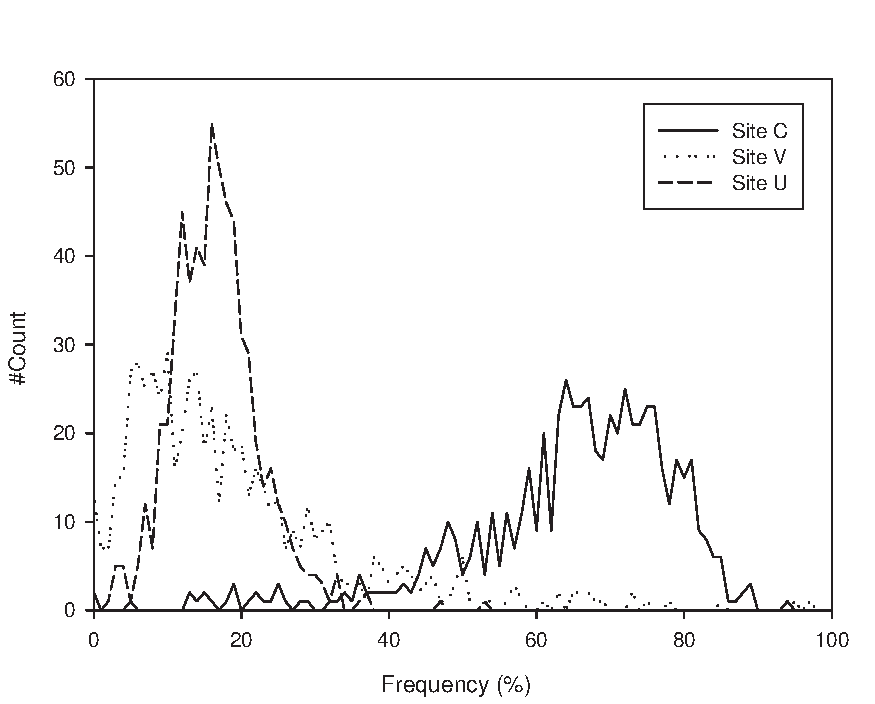
\includegraphics[height=6cm]{figsamp}
\caption{数据曲线图示例}
\label{fig:sample}
\end{figure}

\subsection{表格}

使用浮动环境 \verb|table| 的示例见表\ref{tab:sample}。
\begin{table}
  \caption{表格示例}
  \label{tab:sample}
  \centering
  \begin{tabular}{lcr}%{|l|c|r|}
    \hline
    求解算法                & 系数矩阵的规模    & 执行时间(秒)  \\
    \hline
    Gauss消去法(直接法)     & Mat1903           &  113.27       \\
    Jacobi点迭代            & Mat1784           &  201.36       \\
    \hline
  \end{tabular}
\end{table}

\subsection{数学公式}

本模板提供的文档类 \verb|csoarticle| 本身默认情况下已经包含了 \verb|amsmath| 和 \verb|amsthm| 宏包,因此可以使用这些宏包中提供的一切命令。带编号的数学公式建议使用 \verb|align| 环境。举例如下:一元二次方程
\begin{align}\label{eq:sample}
    a x^2 + b x + c = 0
\end{align}
的两个根为
\begin{align}\label{eq:root}
    x_1 &= \frac{-b + \sqrt{b^2 - 4ac}}{2a} \\
    x_2 &= \frac{-b - \sqrt{b^2 - 4ac}}{2a}
\end{align}
其中,方程\eqref{eq:sample}中的系数$a \not= 0$。

数学类内容中常用的定理类环境也可以直接使用,举例如下(\emph{均为虚拟例子,切勿进行技术性探究}):
\begin{lemma}\label{lem:levy}
    引理的具体内容。
\end{lemma}
\begin{proof}
    可参看各类数学分析类教材,此处从略。
\end{proof}

\begin{theorem}[牛顿第二定律]\label{thm:newton}
物体的质量$m$、物体所受的力$F$以及物体运动的加速度$a$之间满足
\begin{align}\label{eq:f-eq-ma}
    F = m a
\end{align}
\end{theorem}
\begin{proof}
由引理\ref{lem:levy}及文献\cite{bib1}第15章的定理4可立得。
\end{proof}

请直接查看以上例子的源代码部分。

\subsection{参考文献的格式要求}

文献数量应不低于6篇,综述文章文献数量不低于25篇。

注:文中所引的参考文献, 作者均应认真阅读过, 对文献的作者、题目、发表的刊物、年份、卷期号和起止页码等均应核实无误,并按在正文出现的先后顺序编号。标引的序号两边加“[ ]”,作者不超过3人的姓名都写, 超过3人的第三人后面加“,等(et al)” 。无论中外署名,一律姓(大写)先名后,作者姓名之间以逗号分隔。参考文献一律置于文末。文献正文中所有非英文文献需写出对应的英文译文,具体格式要求如下(例子请参看本模板文后的参考文献):
\begin{enumerate}
\item\textbf{期刊:}     作者. 论文题目[J]. 刊名,年,卷(期):起始页码~终止页码.
\item\textbf{专著:}     作者. 书名[M]. 出版地:出版社,出版年.
\item\textbf{译著:}     作者. 书名[M]. 译者. 出版地:出版社,出版年.
\item\textbf{论文集:}   作者. 论文题目[A]. 编者. 文集[C]. 出版地:出版社,出版年. 起始页码~终止页码.
\item\textbf{学位论文:} 作者. 论文题目[D]. 所在城市:保存单位,年份.
\item\textbf{技术标准:} 起草责任者,技术标准代号顺序号—发布年. 技术标准名称[S]. 出版地:出版社,出版年.其中,起草责任者、出版地、出版社、出版年可省。
\item\textbf{专利:}     申请者. 专利名[P]. 国名及专利号,发布日期.
\item\textbf{技术报告:} 作者. 文题[R]. 地名:责任单位,报告代码及编号,年份.
\item\textbf{报纸文章:} 作者. 文题[N]. 报纸名,出版日期(版次).
\item\textbf{在线文献:} 作者. 文题[OL]. [日期]. http://......
\item\textbf{光盘文献:} 作者. 文题[CD]. 出版地:出版者,出版日期.
\item\textbf{其他文献:} 作者. 文题[Z]. 出版地:出版者,出版日期.
\end{enumerate}

\section{结论}

本文给出了………

\section*{致谢(可选)}

应向对论文有帮助的有关人士或单位表示谢意。


%----------------------------------------------------------
% 3. 参考文献
%----------------------------------------------------------

\begin{thebibliography}{2} % 这里的2是指参考文献总数目,需要根据实际情况进行修改
    \bibitem{bib1} H.E.S.Said, T.Tan and K.Baker.Personal identification based on handwriting [J].Pattern Recognition, 33:149-160, Jan. 2000
    \bibitem{bib2} 吴佑寿,丁晓青.汉字识别原理与应用[M],北京:高等教育出版社,1992.8
\end{thebibliography}

\end{document}
